%% ------------------------------------------------------------------------- %%
\section{Análise Espectral}
\label{sec:fourier}

A \emph{Transformada de Fourier} é o passo mais básico para muitos dos algoritmos de transcrição melódica. Ela decompõe uma função periódica em suas senóides constituintes (\emph{parciais}), como pode ser visto na figura \ref{fig:fourier3}.
%\newline

\begin{figure}%[!htb]
\centering
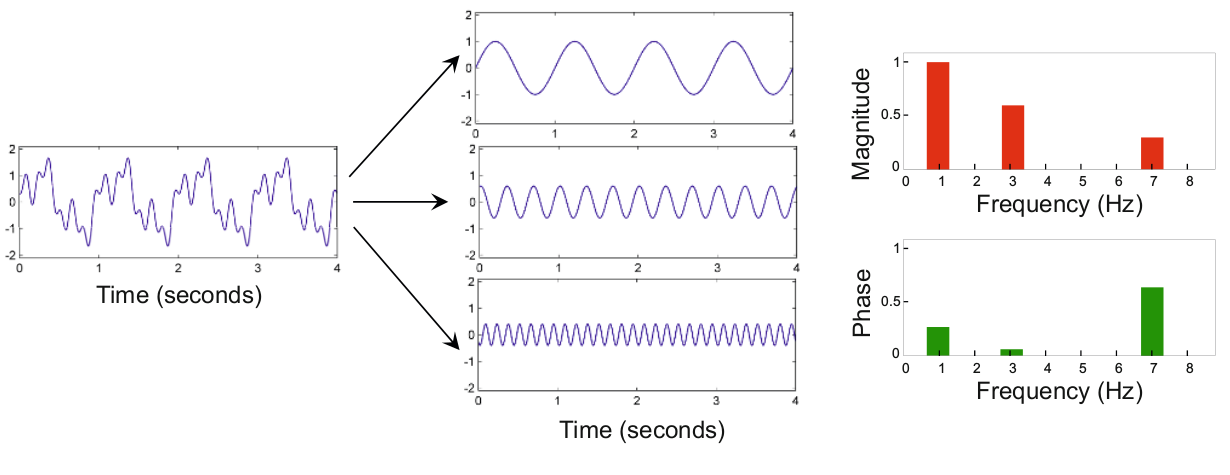
\includegraphics[width=0.9\linewidth]{fourier3}
\caption{Decomposição de um sinal em três parciais.}
\label{fig:fourier3}
\end{figure}

Se dividirmos o nosso sinal temporal em \emph{janelas} de tempo com $N$ amostras obtidas a partir de uma taxa amostral $R$, podemos utilizar um algoritmo de Transformada Discreta de Fourier para conseguir uma matriz onde cada coluna representa a Transformada de Fourier de uma dessas janelas e cada linha representa um \emph{escaninho} de $R/N$ Hz. Se escolhermos uma janela de $N=2^k$ amostras, podemos utilizar o algoritmo de Transformada Rápida de Fourier, cujo tempo de execução é $O(N\log{}N)$.
%\newline

A Transformada de Fourier aplicada à um sinal de áudio pode ser vista na figura \ref{fig:fourier}.

\begin{figure}%[!htb]
\centering
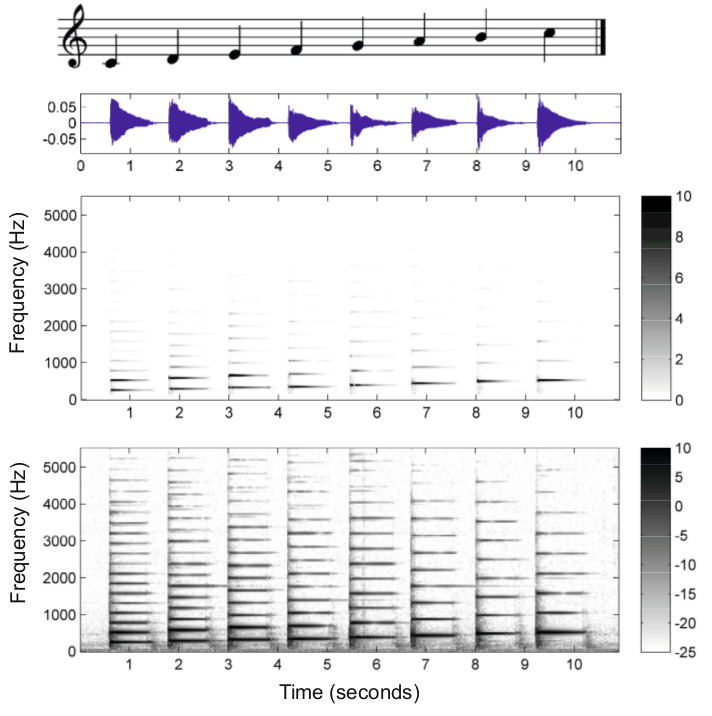
\includegraphics[width=0.6\linewidth]{fourier}
\caption{Transformada de Fourier em um sinal de áudio obtido a partir de um piano.}
\label{fig:fourier}
\end{figure}

%\begin{itemize}
%\item Explicar o que é um som harmônico e o modelo do sinal
%\item Explicar o que é domínio do tempo e domínio de frequência e a transformada de Fourier
%\item Colocar bastantes figuras: Partitura -> Som -> sinal digital (domínio do tempo) -> sinal digital (domínio da frequência) -> transcrição melódica (estimativa de F0)
%\end{itemize}
